\documentclass[aspectratio=169,11pt,svgnames]{beamer}

\usepackage[english]{babel}
\usepackage{graphicx}
\usepackage{enumitem}
\setlist[itemize,1]{label=\textbullet}
\setlist[itemize,2]{label=$\circ$}
\usepackage{amsmath}
\usepackage{mathtools}
\usepackage{float}
\usepackage{tikz}
\usetikzlibrary{patterns,arrows.meta}
\usepackage{tkz-euclide}
\tikzset{point style/.style = {%
  draw = black,
  inner sep = 0pt,
  shape = circle,
  minimum size = 5pt,
  fill = black
 }
}
\usepackage{booktabs} 
\usepackage{pgfplots}
\pgfplotsset{compat=1.18}
\usepackage{pgf-pie}

\usepackage{enumitem}

\usepackage{caption}
\usepackage{subcaption}

% Flowchart stuff

\usepackage{pgfopts}
\usepackage{xcolor}
\usepackage{tcolorbox}

\usetheme[
 titlestyle=style2,
 titleformat=smallcaps,
 sectionstyle=plain,
 slidestyle=cyber,
 headingcolor=theme,
 block=transparent
]{trigon}

\title{Statistics}
\date{\today}
\author{Adam Klepáč}
\institute[GEVO]{Gymnázium Evolution Jižní Město}
\biglogo[width=.2\textwidth]{logo}
\smalllogo[width=.1\textwidth]{logo}
\titlegraphic{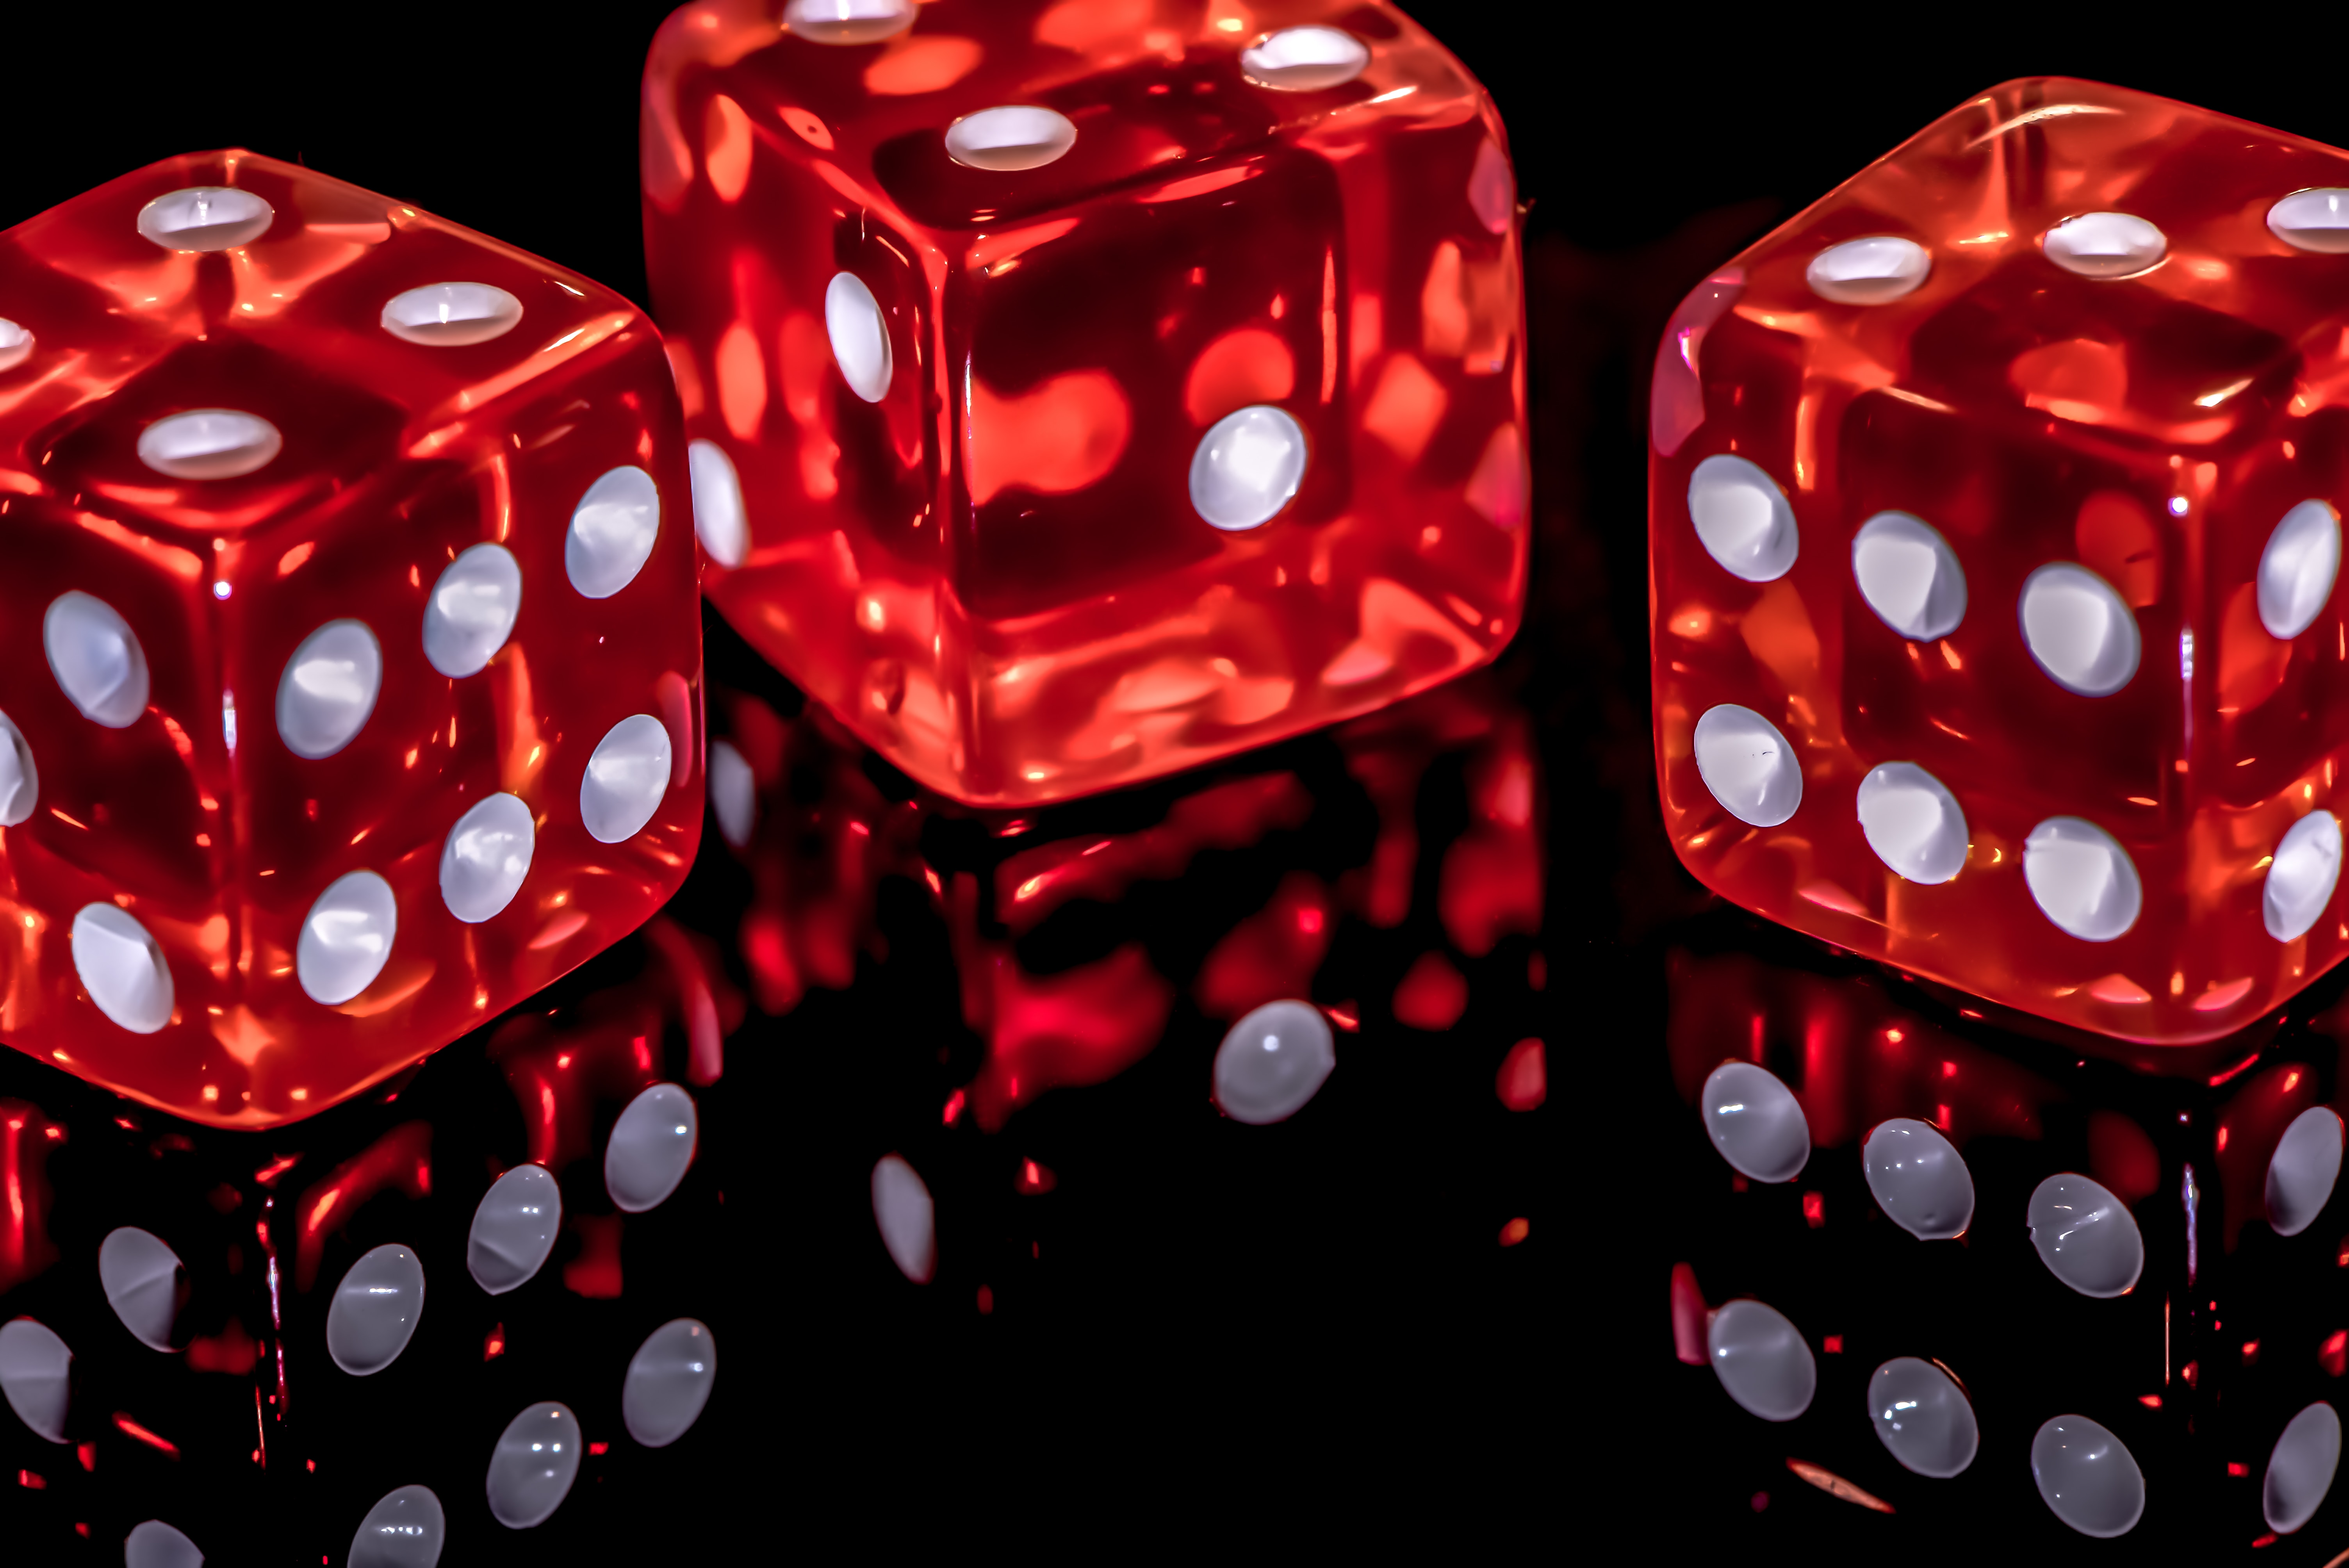
\includegraphics[height=\paperheight]{title.jpg}}

\def\subsectionname{}

% enumerate global settings
\setlist[enumerate,1]{label=\arabic*.}
\setlist[enumerate,2]{label=\alph*)}

% custom colors %
\definecolor{MyTeal}{HTML}{64CCC5}
\definecolor{MyNavy}{HTML}{053B50}
\definecolor{MyBlue}{HTML}{176B87}
\definecolor{MyWhite}{HTML}{EEEEEE}
\colorlet{tPrim}{MyTeal}
\colorlet{tTheme}{MyTeal}
\colorlet{tSec}{MyNavy}
\colorlet{tAccent}{MyBlue}

\tcbset{
 boxsep=7pt,
 fonttitle=\sc,
 colframe=tGreyBg,
 colframe=tPrim,
 boxrule=1pt
}

\newcommand{\clt}{\textcolor{MyTeal}}
\newcommand{\cln}{\textcolor{MyNavy}}
\newcommand{\clb}{\textcolor{MyBlue}}
\newcommand{\clw}{\textcolor{MyWhite}}

\begin{document}
\titleframe

\begin{frame}
 \frametitle{What Even Is Statistics?}
 \begin{tcolorbox}[title=Statistics]
  \alert{Statistics} is a mathematical discipline concerned with predicting
  future state of a system based \emph{solely} on its past behaviour.
 \end{tcolorbox}
 \pause
 The collective information about a system's past state is called
 \alert{data}.\\
 \pause
 It assigns \alert{probabilities} to each possible future state of system based
 on data.\\
 \pause
 It also assigns probabilities to the \alert{possibility of wrong prediction}.
\end{frame}

\begin{frame}
 \frametitle{Example -- Biased Coin?}
 We throw a coin 10 times with the following outcome:
 \[
  \{H,H,H,T,H,T,H,H,H,T\},
 \]
 $H$ for `heads', $T$ for `tails'.
 \pause
 We can ask two questions:
 \pause
 \begin{itemize}[label=\textbullet]
  \item<3-> What is the probability that the \alert{next toss} will come out
   `heads'/`tails'?
  \begin{itemize}[label=\textminus]
   \item<5-> We got $7$ heads out of $10$ tosses, so the probability for the next toss
    being heads is $7 / 10$.
  \end{itemize}
  \item<4-> Is this coin is \alert{biased towards} `heads'/`tails' with
   \emph{allowed probability of error} $\alpha$?
   \begin{itemize}[label=\textminus]
    \item<6-> \alert{No}, for $\alpha = 0.05$.
    \item<6-> \alert{Yes}, for $\alpha = 0.2$.
   \end{itemize}
 \end{itemize}
\end{frame}

\begin{frame}
 \frametitle{Contents}
 \tableofcontents
\end{frame}

\section{Data}

\begin{frame}
 \frametitle{What Do We Mean By Data?}
 \begin{tcolorbox}[title=Data]
  \alert{Sets} (called \emph{inputs} and \emph{outputs}) describing the studied
  system. There is typically only one set of inputs and possibly multiple sets
  of outputs.
 \end{tcolorbox}
\end{frame}

\begin{frame}
 \frametitle{Example -- Junctions}
 For a year, we keep track of the number of traffic accidents per day on road
 junctions across the city to determine which should be first replaced by
 roundabouts.\\
 \pause
 An \alert{input} is a day in a year coupled with the location of the
 junction.\\
 \pause
 An \alert{output} is the number of traffic accidents in the given day on the
 given junction.
\end{frame}

\begin{frame}
 \frametitle{Example -- First Baby}
 We study the age that women bear children for the first time across Europe.\\
 \pause
 An \alert{input} would be a name of a European country.\\
 An \alert{output} is the average age of a first-time mother in that country.
\end{frame}

\subsection{Types of Data}

\begin{frame}
 \subsectionpage
\end{frame}

\begin{frame}
 \frametitle{Discrete Data vs. Continuous Data}
 \begin{tcolorbox}[title=Discrete Data]
  We call a data \alert{discrete} if the set of \emph{inputs} (and therefore also
  that of \emph{outputs}) is \alert{countable}.
 \end{tcolorbox}
 \pause
 Both previous examples feature \alert{discrete} data.
 \begin{itemize}[label=\textbullet]
  \item There are only \emph{finitely many} junctions in a city and days in a
   year.
  \pause
  \item There are only \emph{finitely many} countries on a continent.
 \end{itemize}
\end{frame}

\begin{frame}
 \frametitle{Discrete Data vs. Continuous Data}
 \begin{tcolorbox}[title=Continuous Data]
  We call a data \alert{continuous} if the set of inputs is \alert{uncountable}.
  In this case, the data is actually a \alert{function}: set of inputs $ \to $
  set of outputs.
 \end{tcolorbox}
 \pause
 More often than not, the inputs in a continuous data are \alert{moments in
 time} or \alert{coordinates in space}.
\end{frame}

\begin{frame}
 \frametitle{Continuous Data -- Examples}
 \begin{itemize}[label=\textbullet]
  \item We study the number of trains in a railway station at any given time.
  \pause
  \begin{itemize}[label=\textminus]
   \item Input: time (of day);
   \pause
   \item Output: number of trains in the station.
   \pause
   \item The data is a function $f:[0,24] \to \mathbb{N}$.
  \end{itemize}
 \pause
 \item Another example is the density of air per cubic meter.
 \pause
 \begin{itemize}[label=\textminus] 
  \item Input: Coordinates of a unit cube in space.
  \pause
  \item Output: The combined weight of air molecules.
  \pause
  \item The data is a function $f:\mathbb{R}^3 \to [0,\infty)$. 
 \end{itemize}
 \end{itemize}
\end{frame}

\section{Visualizing Discrete Data}

\begin{frame}
 \frametitle{Tables}
 The simplest possible visualization.\\
 \pause
 You simply write \emph{inputs} into one row/column and \emph{outputs} into the
 other.\\
 \pause
 For example, suppose you measure the height of $10$ random people. You can
 visualize your experiment like this:
 \pause
 \begin{center}
  \begin{tabular}{c|cccccccccc}
   \textbf{Input} & 1 & 2 & 3 & 4 & 5 & 6 & 7 & 8 & 9 & 10\\
   \midrule
   \textbf{Output} & 180 & 169 & 191 & 177 & 175 & 181 & 171 & 153 & 180 & 183
  \end{tabular}
 \end{center}
\end{frame}

\begin{frame}
 \frametitle{Pie Chart}
 Only usable if your outputs \alert{total a predetermined number}, typically
 \emph{percentages}.\\
 \pause
 Suppose we have three inputs --
 $\textcolor{VioletRed}{I_1},\textcolor{Aqua}{I_2}$ and
 $\textcolor{ForestGreen}{I_3}$ -- with three outputs --
 $\textcolor{VioletRed}{30 \%}, \textcolor{Aqua}{10 \%}$ and
 $\textcolor{ForestGreen}{60 \%}$.\\
 \pause
 Pie chart of this data looks like this
 \begin{center}
  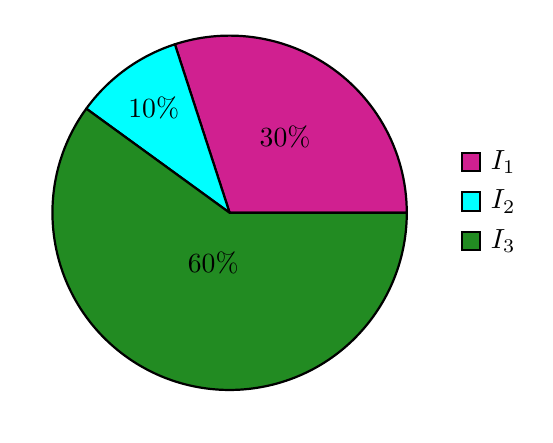
\begin{tikzpicture}[scale=0.75]
   \pie[color={VioletRed,Aqua,ForestGreen},text=legend]{
    30/$I_1$,
    10/$I_2$,
    60/$I_3$
   }
  \end{tikzpicture}
 \end{center}
\end{frame}

\begin{frame}
 \frametitle{Pie Chart -- Examples}
 Pie charts are frequently used to represent compositions of chemicals.\\
 \pause
 For instance, here is a pie chart of the composition of \emph{air}.
 \begin{center}
  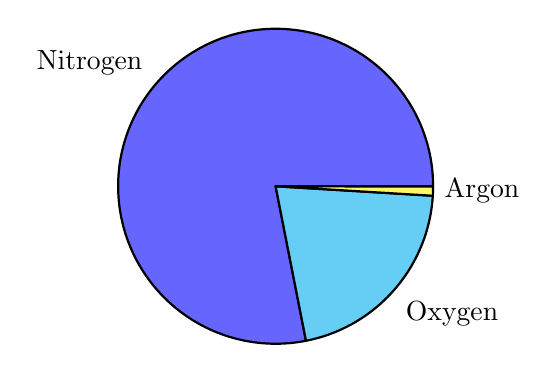
\begin{tikzpicture}
   \pie[hide number,radius=2]{
    78.09/Nitrogen,
    20.95/Oxygen,
    0.93/Argon
   }
  \end{tikzpicture}
 \end{center}
\end{frame}

\begin{frame}
 \frametitle{Pie Chart -- Examples}
 Favourite type of movie as determined by a survey.
 \begin{center}
  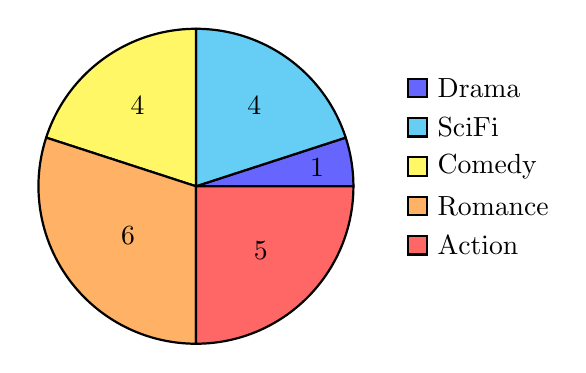
\begin{tikzpicture}
   \pie[radius=2,text=legend,before number=,after number=,sum=20]{
    1/Drama,
    4/SciFi,
    4/Comedy,
    6/Romance,
    5/Action
   }
  \end{tikzpicture}
 \end{center}
\end{frame}

\begin{frame}
 \frametitle{Bar Chart}
 Usable basically for any discrete data.\\
 \pause
 Especially useful when your inputs are ordered and when you expect the data to
 follow a certain trend -- it can be easily approximated by a polygonal curve.\\
 \pause
 Also very good for comparing more outputs for the same inputs.\\
\end{frame}

\begin{frame}
 \frametitle{Bar Chart -- Example}
 Suppose we count the number of customers in our shop over each hour. If we're
 open from 8 AM to 5 PM, a bar chart of such an experiment can look like this:
 \pause
 \begin{center}
  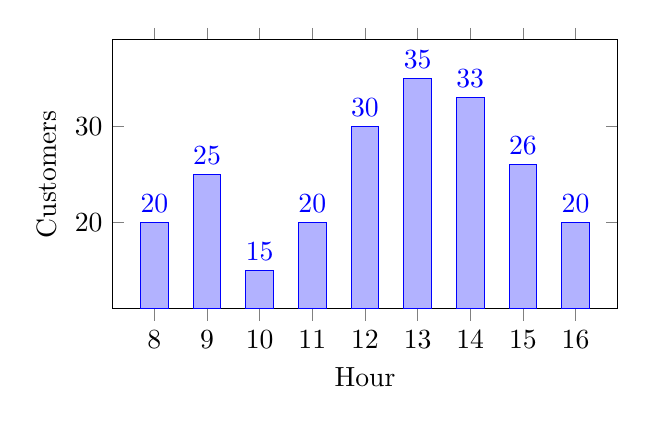
\begin{tikzpicture}
   \begin{axis}[ybar,height=5cm,width=8cm,xmin=8,xmax=16,
    ylabel=Customers,xlabel=Hour,enlarge y limits=0.2,
    enlarge x limits=0.1,nodes near coords,xtick distance=1]
    \addplot coordinates {
      (8,20) (9,25) (10,15) (11,20)
      (12,30) (13,35) (14,33) (15,26) (16,20)
     };
   \end{axis}
  \end{tikzpicture}
 \end{center}
\end{frame}

\begin{frame}
 \frametitle{Bar Chart -- Example}
 Let's say we open another shop and want to compare how the two shops are doing
 at each hour.\\
 \pause
 We can show both outputs in the same bar chart:\\
 \pause
 \begin{center}
  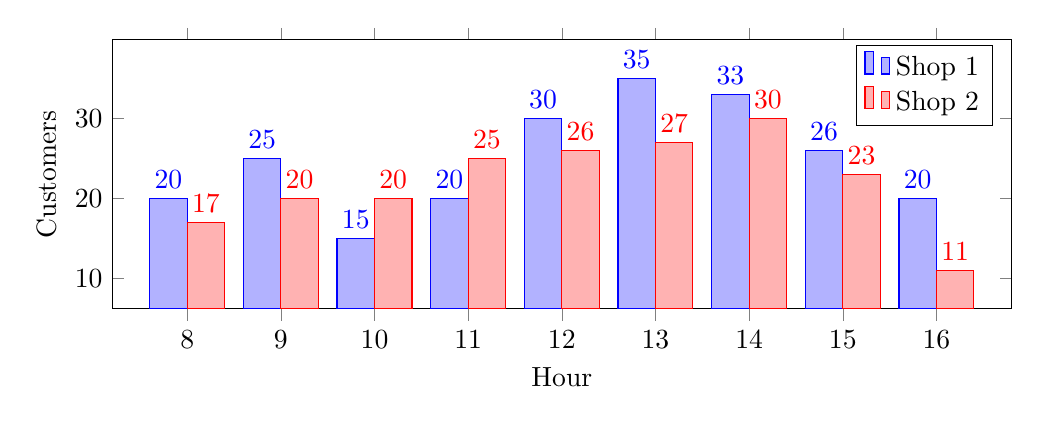
\begin{tikzpicture}
   \begin{axis}[ybar=0pt,height=5cm,width=13cm,xmin=8,xmax=16,
    ylabel=Customers,xlabel=Hour,enlarge y limits=0.2,
    enlarge x limits=0.1,nodes near coords,xtick distance=1,
    bar width=0.4]
    \addplot coordinates {
      (8,20) (9,25) (10,15) (11,20)
      (12,30) (13,35) (14,33) (15,26) (16,20)
     };
    \addplot coordinates {
      (8,17) (9,20) (10,20) (11,25)
      (12,26) (13,27) (14,30) (15,23) (16,11)
     };
    \legend{Shop 1, Shop 2}
   \end{axis}
  \end{tikzpicture}
 \end{center}
\end{frame}

\begin{frame}
 \frametitle{Bar Chart -- Example}
 You can also use bar chart to stack outputs on top of each other.\\
 \pause
 For example, if I wanted to know the \textbf{total} number of customers in both
 my shops, I could draw a chart like this:
 \pause
 \begin{center}
  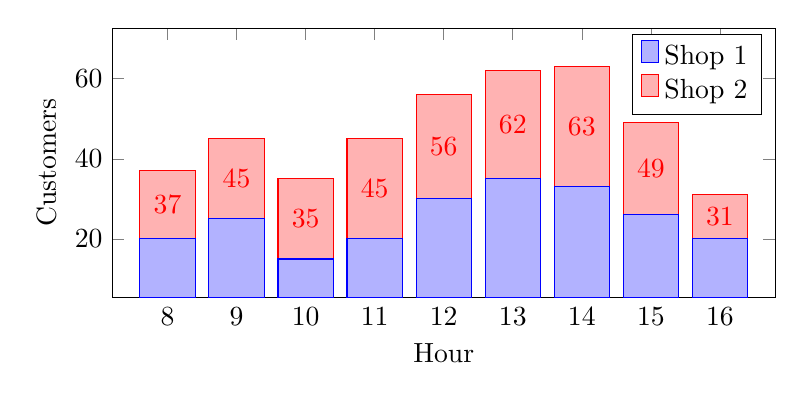
\begin{tikzpicture}
   \begin{axis}[height=5cm,width=10cm,xmin=8,xmax=16,
    ylabel=Customers,xlabel=Hour,enlarge y limits=0.2,
    enlarge x limits=0.1,xtick distance=1,
    bar width=0.8,ybar stacked]
    \addplot coordinates {
      (8,20) (9,25) (10,15) (11,20)
      (12,30) (13,35) (14,33) (15,26) (16,20)
     };
    \addplot +[nodes near coords,point meta=y] coordinates {
      (8,17) (9,20) (10,20) (11,25)
      (12,26) (13,27) (14,30) (15,23) (16,11)
     };
    \legend{Shop 1, Shop 2}
   \end{axis}
  \end{tikzpicture}
 \end{center}
\end{frame}

\begin{frame}
 \frametitle{Scatter Plot}
 Scatter plots are useful when studying `random' data.\\
 \pause
 Something like the position of an air molecule in a box over time.\\
 \pause
 \begin{center}
  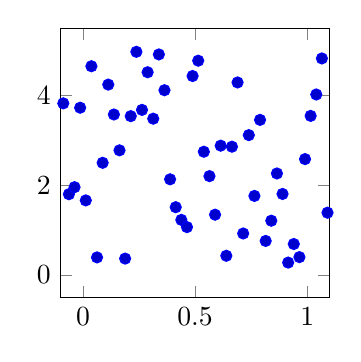
\begin{tikzpicture}
   \begin{axis}[height=5cm,width=5cm,enlargelimits=0.1,
    xmin=0,xmax=1,ymin=0,ymax=5]
    \addplot+ [
     only marks,
     samples=400
    ] {2.5*(rand + 1)};
   \end{axis}
  \end{tikzpicture}
 \end{center}
 \vspace*{-1em}
 Here, the $x$-axis represents time (0 to 1s) and the $y$-axis represents one
 coordinate of the molecule (say the box is a 5x5x5 cube).
\end{frame}

\begin{frame}
 \frametitle{Scatter Plot -- Example}
 Of course, you can also display multiple outputs with the same inputs in a
 scatter plot.\\
 \pause
 Let's add another air molecule.\\
 \pause
 \begin{center}
  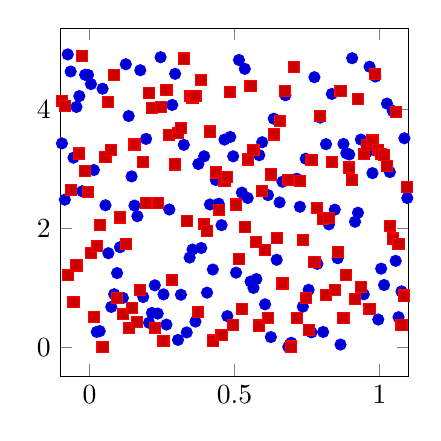
\begin{tikzpicture}
   \begin{axis}[height=6cm,width=6cm,enlargelimits=0.1,
    xmin=0,xmax=1]
    \addplot+ [
     only marks,
     samples=1000
    ] {2.5*(rand + 1)};
    \addplot+ [
     only marks,
     samples=1000
    ] {2.5*(rand + 1)};
   \end{axis}
  \end{tikzpicture}
 \end{center}
\end{frame}

\section{Mean -- Median -- Deviation -- Correlation}

\begin{frame}
 \frametitle{Useful Values}
 When studying data, there are \alert{certain numerical values} which prove
 useful in predicting future behaviour.\\
 \pause
 Facts we wish to learn about our data include:
 \pause
 \begin{itemize}[label=\textbullet]
  \item the expected value of the next experiment (the \alert{mean}),
  \pause
  \item the `middle' value of the outputs regardless of proportion (the
   \alert{median}),
  \pause
  \item the expected/observed measure of difference of observed values from the
   mean (the \alert{deviation}),
  \pause
  \item dependence on any other data (the \alert{correlation}).
 \end{itemize}
\end{frame}

\subsection{The Mean}

\begin{frame}
 \subsectionpage
\end{frame}

\begin{frame}
 \frametitle{Types of Mean}
 The \alert{mean} in some sense is `the most probable' next output based on the
 received data.\\
 \pause
 What is `the most probable' output however depends heavily on the type of
 experiment we are performing.\\
\end{frame}

\begin{frame}
 \frametitle{Types of Mean -- Arithmetic Mean}
 \begin{tcolorbox}[title=Arithmetic Mean]
  The \alert{arithmetic mean} is the sum of outputs divided by their number. If
  $x_1,\ldots,x_n$ are the outputs, their arithmetic mean (often denoted
  $\bar{x}$) is
  \[
   \bar{x} \coloneqq \frac{x_1+x_2+\ldots +x_n}{n}.
  \]
 \end{tcolorbox}
 \pause
 Most useful when dealing with data in \alert{absolute} proportion.\\
 \pause
 Meaning that we're interested in `\alert{how much}' is one output
 smaller/larger than another.
\end{frame}

\begin{frame}
 \frametitle{Arithmetic Mean -- Example}
 The arithmetic mean is for most experiments the relevant one.\\
 \pause
 Consider for example an experiment tailored to determine the average height of
 a $15$-year-old British male.\\
 \pause
 While comparing the heights of two people, we care about the \alert{absolute}
 difference in centimetres.\\
 \pause
 For example, if this is our data
 \begin{center}
  \begin{tabular}{c|ccccc}
   \textbf{Input} & 1 & 2 & 3 & 4 & 5\\
   \midrule
   \textbf{Output} & 165 & 161 & 164 & 172 & 168,
  \end{tabular}
 \end{center}
 we conclude that the expected height of a randomly chosen $15$-year-old British
 male is
 \[
  \frac{165 + 161 + 164 + 172 + 168}{5} = 166.
 \]
\end{frame}

\begin{frame}
 \frametitle{Types of Mean -- Geometric Mean}
 \begin{tcolorbox}[title=Geometric Mean]
  The \alert{geometric mean} is the $n$-th root of the product of $n$ outputs.
  That is, if $x_1,\ldots,x_n$ are the outputs, their geometric mean is
  \[
   \bar{x} \coloneqq \sqrt[n]{(x_1 \cdot x_2 \cdot \ldots \cdot x_n)}.
  \]
 \end{tcolorbox}
 \pause
 Most useful when dealing with data in \alert{relative} proportion.\\
 \pause
 Meaning that we're interested in `\alert{how many times}' is one output
 smaller/larger than another.
\end{frame}

\begin{frame}
 \frametitle{Geometric Mean -- Example}
 Suppose we're comparing the increase in population in Asian countries since the
 year 2000.\\
 \pause
 When comparing two populations, we don't really care \emph{by how much} they
 differ, but \emph{how many times} is one larger than the other.\\
 \pause
 If this is our data
 \begin{center}
  \begin{tabular}{c|cccccc}
   \textbf{Input} & India & China & Japan & South Korea & Mongolia & Taiwan\\
   \midrule
   \textbf{Output} & 1.328 & 1.118 & 0.991 & 1.100 & 1.366 & 1.078
  \end{tabular}
 \end{center}
 then the expected increase in population in a randomly chosen Asian country is
 \[
  \sqrt[6]{(1.328 \cdot 1.118 \cdot 0.991 \cdot 1.100 \cdot 1.366 \cdot 1.078)}
  = 1.156.
 \]
\end{frame}

\begin{frame}
 \frametitle{Types of Mean -- Harmonic Mean}
 \begin{tcolorbox}[title=Harmonic Mean]
  The \alert{harmonic mean} is the reciprocal of the sum of reciprocals divided
  by their number. If $x_1,\ldots,x_n$ are the outputs, their harmonic mean is
  \[
   \bar{x} \coloneqq \frac{n}{\frac{1}{x_1} + \frac{1}{x_2}
   +\ldots+\frac{1}{x_n}}.
  \]
 \end{tcolorbox}
 \pause
 Most useful when dealing with \alert{rates} and \alert{ratios}.\\
 \pause
 Meaning when comparing outputs which are actually ratios of two numbers.
\end{frame}

\begin{frame}
 \frametitle{Harmonic Mean -- Example}
 We study the speed of a train between individual stations.\\
 \pause
 If this is our data
 \begin{center}
  \begin{tabular}{c|cccccc}
   \textbf{Input} & $1 \to 2$ & $2 \to 3$ & $3 \to 4$ & $4 \to 5$ & $5 \to 6$ &
   $6 \to 7$\\
   \midrule
   \textbf{Output} & 65 km/h & 52 km/h & 71 km/h & 60 km/h & 62 km/h & 53 km/h,
  \end{tabular}
 \end{center}
 then the average speed of the train over the whole track is
 \[
  \frac{6}{\frac{1}{65} + \frac{1}{52} + \frac{1}{71} + \frac{1}{60} +
  \frac{1}{62} + \frac{1}{53}} = 59.78 \text{ km/h}.
 \]
 \pause
 Actually, here the arithmetic mean is 60.5 km/h which is not just an
 \emph{inadequate} estimate, it's simply \textbf{the wrong answer!}\\
 \pause
 If you summed up all the distances between stations and divided them by the
 total time, you would get the \textbf{harmonic mean!}
\end{frame}

\subsection{The Median}
\begin{frame}
 \frametitle{}
 \subsectionpage
\end{frame}

\begin{frame}
 \frametitle{The Median}
 \begin{tcolorbox}[title=Median]
  The \alert{median} is the value which lies exactly in the middle of a dataset.
  It is essentially the value separating the lower and upper half of outputs. If
  $x_1,\ldots,x_n$ are the outputs \alert{ordered from least to greatest}, the
  median is
  \[
   \mathrm{median}(x) \coloneqq 
   \begin{cases}
    x_{(n+1) / 2} & \text{ if } $n$ \text{ is odd},\\
    \frac{x_{n / 2} + x_{n / 2 + 1}}{2} & \text{ if } $n$ \text{ is even}.
   \end{cases}
  \]
 \end{tcolorbox}
\end{frame}

\begin{frame}
 \frametitle{The Median -- Example}
 The median is useful when dealing with data manifesting radical extremes.\\
 \pause
 It is very often used in relationship to \alert{location}.\\
 \pause
 For example, imagine we're trying to determine the distance from our measuring
 station to the hypocentre of an earthquake.\\
 \pause
 We can detect where the quake is strongest, giving us this data:
 \begin{center}
  \begin{tabular}{c|cccccc}
   \textbf{Input} & 1 & 2 & 3 & 4 & 5 & 6\\
   \midrule
   \textbf{Output} & 1 km & 2 km & 2 km & 2 km & 3 km & 14 km
  \end{tabular}
 \end{center}
 \pause
 The median of this dataset is 2 km which is a much better estimate of a
 `centre' than for example the arithmetic mean, being equal to $4$, is.\\
 \pause
 Also, the mean and the median cannot be `too far' apart and the median requires
 at most two values to calculate, making it a very resource efficient
 approximation of the mean.
\end{frame}

\subsection{The Deviation}
\begin{frame}
 \frametitle{}
 \subsectionpage
\end{frame}

\begin{frame}
 \frametitle{Deviation}
 \begin{tcolorbox}[title=Deviation]
  \alert{Deviation} is a measure of the difference between the observed outputs
  and the computed mean.
 \end{tcolorbox}
 \pause
 There are many types of deviations, we'll focus on two of them:
 \pause
 \begin{itemize}[label=\textbullet]
  \item the \alert{standard deviation} (a measure of `dispersion'),
  \pause
  \item the \alert{average absolute deviation} (a measure of actual
   `difference').
 \end{itemize}
 \pause
 A \alert{very important distinction} is that the \emph{standard deviation}
 concerns \textbf{future} measurements while the \emph{average absolute
 deviation} concerns \textbf{past} measurements.
\end{frame}

\begin{frame}
 \frametitle{Types of Deviation -- Standard Deviation}
 \begin{tcolorbox}[title=Standard Deviation]
  The \alert{standard deviation} measures the dispersion of a set of values.
  Basically, it measures how likely the data is to concentrate around the mean.
  If $x_1,\ldots,x_n$ are the outputs and $\bar{x}$ is their \textbf{arithmetic}
  mean, then their standard deviation is
  \[
   \sigma \coloneqq \sqrt{\frac{1}{n}((x_1-\bar{x})^2 +
   (x_2-\bar{x})^2+\ldots+(x_n-\bar{x})^2)}.
  \]
 \end{tcolorbox}
\end{frame}

\begin{frame}
 \frametitle{Standard Deviation -- Example}
 Let us repeat the height experiment. We measured the heights of 5 $15$-year-old
 British males to try to determine the national average. This is the data:
 \begin{center}
  \begin{tabular}{c|ccccc}
   \textbf{Input} & 1 & 2 & 3 & 4 & 5\\
   \midrule
   \textbf{Output} & 165 & 161 & 164 & 172 & 168
  \end{tabular}
 \end{center}
 \pause
 We computed the arithmetic mean to be 166. This means that the standard
 deviation of this data is
 \begin{align*}
  \sigma &= \sqrt{\frac{1}{5}((165 - 166)^2 + (161 -166)^2 + (164 - 166)^2 +
  (172-166)^2 + (168-166)^2)}\\
         &= 3.742,
 \end{align*}
 meaning we can expect most new values to concentrate 3.742 cm around 166 cm.
\end{frame}

\begin{frame}
 \frametitle{Types of Deviation -- Average Absolute Deviation}
 \begin{tcolorbox}[title=Average Absolute Deviation]
  The \alert{average absolute deviation} is the average of the absolute
  deviations from a chosen central point (typically the mean). If
  $x_1,\ldots,x_n$ are the outputs and $\bar{x}$ is the chosen central point,
  then the average absolute deviation of this dataset is
  \[
   \frac{|x_1 - \bar{x}| + |x_2 - \bar{x}| + \ldots + |x_n -\bar{x}|}{n}.
  \]
 \end{tcolorbox}
\end{frame}

\begin{frame}
 \frametitle{Average Absolute Deviation -- Example}
 If we return to the height experiment yet again, we can calculate that the
 average absolute deviation of the data (with the central point being the
 arithmetic mean)
 \begin{center}
  \begin{tabular}{c|ccccc}
   \textbf{Input} & 1 & 2 & 3 & 4 & 5\\
   \midrule
   \textbf{Output} & 165 & 161 & 164 & 172 & 168
  \end{tabular}
 \end{center}
 \pause
 is
 \[
  \frac{|165 - 166| + |161 - 166| + |164 - 166| + |172 - 166| + |168 - 166|}{5}
  = 3.2,
 \]
 \pause
 meaning that the measured heights differ on average by 3.2 cm from the
 calculated arithmetic mean.
\end{frame}

\subsection{Correlation}
\begin{frame}
 \frametitle{}
 \subsectionpage
\end{frame}

\begin{frame}
 \frametitle{Correlation}
 \begin{tcolorbox}[title=Correlation]
  \alert{Correlation} or \alert{dependence} is a relationship between two
  outputs of a dataset. A `correlation' in many cases means some type of
  association.
 \end{tcolorbox}
 \pause
 Correlation is an number between $-1$ and $1$.
 \pause
 Intuitively, a
 \begin{itemize}[label=\textbullet]
  \item negative correlation means that the two series of outputs
   \alert{contradict} each other;
  \pause
  \item zero correlation means that the two series of outputs are
   \alert{unrelated};
  \pause
  \item positive correlation means that the two series of outputs
   \alert{influence} each other.
 \end{itemize}
\end{frame}

\begin{frame}
 \frametitle{Computing Correlation}
 \begin{tcolorbox}[title=Correlation Formula]
  If $x_1,\ldots,x_n$ and $y_1,\ldots,y_n$ are two series of outputs for the
  same inputs with means $\bar{x}$ and $\bar{y}$, their correlation is
  \[
   \mathrm{cor}(x,y) \coloneqq \frac{(x_1-\bar{x})(x_2-\bar{x})\cdots
   (x_n-\bar{x})(y_1-\bar{y})(y_2-\bar{y})\cdots
  (y_n-\bar{y})}{\sqrt{(x_1-\bar{x})^2(x_2-\bar{x})^2\cdots
 (x_n-\bar{x})^2(y_1-\bar{y})^2(y_2-\bar{y})^2\cdots (y_n-\bar{y})^2}}.
  \]
 \end{tcolorbox}
\end{frame}

\begin{frame}
 \frametitle{Interpreting Correlation -- Table}
 A crude interpretation of correlation is given in the following table:
 \begin{center}
  \begin{tabular}{ccc}
   \textbf{Coefficient} & \textbf{Strength} & \textbf{Type} \\
   \toprule
   -0.7 to -1 & Very strong & Negative\\
   -0.5 to -0.7 & Strong & Negative\\
   -0.3 to -0.5 & Moderate & Negative\\
   0 to -0.3 & Weak & Negative\\
   0 to 0.3 & Weak & Positive\\
   0.3 to 0.5 & Moderate & Positive\\
   0.5 to 0.7 & Strong & Positive\\
   0.7 to 1 & Very strong & Positive
  \end{tabular}
 \end{center}
\end{frame}

\begin{frame}
 \frametitle{Interpreting Correlation -- Chart}
 You can use a scatter plot to visualize two sets of outputs with the same
 inputs.
 \pause
 Correlation tells you \alert{how well you can approximate} this scatter plot by
 a straight line.
 \pause
 For example, imagine you measure the height and weight of a sample of people
 and want to see if they correlate. You might get a scatter plot like this:
 \pause
 \begin{center}
  \begin{tikzpicture}
   \begin{axis}[height=5cm,width=6cm]
    \addplot+[
     only marks,
     scatter]
     table[meta=height]
     {correlation.dat};
   \end{axis}
  \end{tikzpicture}
 \end{center}
\end{frame}

\section{Frequency Distribution}

\begin{frame}
 \frametitle{What Is Frequency Distribution?}
 \begin{tcolorbox}[title=Frequency Distribution]
  A \alert{frequency} of a value is the number of times it occurs in a dataset.
  A \alert{frequency distribution} is the number of times each variable occurs
  in a dataset.
 \end{tcolorbox}
\end{frame}

\begin{frame}
 \frametitle{Types of Frequency Distributions}
 \begin{itemize}[label=\textbullet]
  \item \alert{Ungrouped frequency distribution}: the number of observations of
   each output. It's usable for \emph{categorical data}.
  \pause
  \item \alert{Grouped frequency distribution}: the number of observations of
   each \textbf{class interval} of a variable. Useful for \emph{quantitative
   data}.
  \pause
  \item \alert{Relative frequency distribution}: the proportion of each value or
   class interval of a variable. Useful for any type of data \textbf{if we care
   about comparing frequencies} rather than amounts.
  \pause
  \item \alert{Cumulative frequency distribution}: the sum of frequencies less
   than or equal to each value or class interval of a variable. Useful when we
   want to understand how often observations fall below certain values.
 \end{itemize}
\end{frame}

\begin{frame}
 \frametitle{Categorical vs Quantitative Data}
 \alert{Quantitative Data} represent real amounts that can be added, subtracted
 etc.
 \pause
 \begin{itemize}[label=\textbullet]
  \item Can be discrete or continuous:
  \pause
  \begin{itemize}[label=$\circ$]
   \item \textbf{Discrete data} represents counts of individual items like number of
    students in a class.
   \pause
   \item \textbf{Continuous data} represents measurements of uncountable values like
    density, volume or time.
  \end{itemize}
 \end{itemize}
\end{frame}

\begin{frame}
 \frametitle{Categorical vs Quantitative Data}
 \alert{Categorical Data} represents groupings. They can be recorded as numbers
 but the numbers represent categories and not actual amounts.
 \pause
 \begin{itemize}[label=\textbullet]
  \item Can be binary, nominal or ordinal:
  \pause
  \begin{itemize}[label=$\circ$]
   \item \textbf{Binary data} represents yes or no outcomes like coin flips or
    win/loss situations.
   \pause
   \item \textbf{Nominal data} represents groups without rank or order between
    them -- like the names of species or colours.
   \pause
   \item \textbf{Ordinal data} represents groups that are ranked -- like
    finishing place in a race.
  \end{itemize}
 \end{itemize}
\end{frame}

\begin{frame}
 \frametitle{Ungrouped Frequency Data -- Table}
 \begin{enumerate}
  \item Create a table with one column for inputs and as many columns as there
   are output with a row for each input.
   \pause
   \begin{itemize}
    \item For \alert{ordinal} variables, the values should be ordered from
     smallest to largest.
    \pause
    \item For \alert{nominal} variables, the rows can be ordered arbitrarily.
   \end{itemize}
  \item Count the \alert{frequencies}.
 \end{enumerate}
\end{frame}

\begin{frame}
 \frametitle{Ungrouped Frequency Data -- Example 1}
 A gardener sets up a bird feeder in his backyard. He wishes to know which type
 of bird species visit the feeder the most.
 \pause
 His observations are in the following table:
 \begin{center}
  \begin{tabular}{c|c}
   \textbf{Species} & \textbf{Frequency}\\
   \toprule
   Chickadee & 3\\
   Dove & 1\\
   Finch & 4\\
   Grackle & 2\\
   Sparrow & 4\\
   Starling & 2
  \end{tabular}
 \end{center}
\end{frame}

\begin{frame}
 \frametitle{Ungrouped Frequency Data -- Example 2}
 We observe how many times a specific type of tram (based on age) stops at a
 chosen station each day.\\
 \pause
 This experiment may yield a table like this:
 \begin{center}
  \begin{tabular}{c|c}
   \textbf{Type} & \textbf{Frequency}\\
   \toprule
   1990 & 6\\
   1996 & 11\\
   2005 & 3\\
   2017 & 5
  \end{tabular}
 \end{center}
\end{frame}

\begin{frame}
 \frametitle{Grouped Frequency Data -- Table}
 \begin{enumerate}
  \item Divide the variables into \alert{class intervals}. There's no `best
   choice' for the width of a class interval. Different choices convey different
   meanings.
   \pause
   \begin{itemize}
    \item Calculate the \alert{range} = $\text{highest value} - \text{lowest
     value}$.
    \pause
    \item Decide on the \alert{class interval width}. \textbf{ALWAYS THINK}
     about that the best width should be! But, if you can't decide, a rule of
     thumb is the width
     \[
      \text{width} = \frac{\text{range}}{\sqrt{\text{number of inputs}}}.
     \]
     It is typically beneficial to round this value to an integer.
    \pause
    \item Calculate the \alert{class intervals}. Each interval is of the form
     $[\text{lower limit}, \text{lower limit} + \text{width})$. Simply divide
     the outputs into these intervals.
   \end{itemize}
 \end{enumerate}
\end{frame}

\begin{frame}
 \frametitle{Grouped Frequency Data -- Table}
 \begin{enumerate}
  \setcounter{enumi}{1}
  \item Create a \alert{table} with columns for inputs and each output and as
   many rows as there are class intervals.
  \pause
  \item Count the \alert{frequencies}.
 \end{enumerate}
\end{frame}

\begin{frame}
 \frametitle{Grouped Frequency Data -- Example}
 In sociological surveys, you typically want to find the distribution of
 respondents by age.\\
 \pause
 Let's say a survey had 20 respondents. Their ages go like this:
 \[
  52, 34, 32, 29, 63, 40, 46, 54, 36, 36, 24, 19, 45, 20, 28, 29, 38, 33, 49,
  37.
 \]
 \pause
 We calculate the range as $\text{highest} - \text{lowest} = 63 - 19 = 44$.\\
 We calculate the interval width as
 \[
  \text{width} = \frac{\text{range}}{\sqrt{\text{sample size}}} =
  \frac{44}{\sqrt{20}} = 9.84,
 \]
 and round it up to $10$.\\
 \pause
 Therefore, we have the following intervals
 \[
  [19, 29), [29, 39), [39, 49), [49, 59), [59, 69).
 \]
\end{frame}

\begin{frame}
 \frametitle{Grouped Frequency Data -- Example}
 Counting the numbers of outputs falling into each of those intervals gives the
 table:
 \begin{center}
  \begin{tabular}{c|c}
   \textbf{Age} & \textbf{Frequency}\\
   \toprule
   19 -- 28 & 4\\
   29 -- 38 & 9\\
   39 -- 48 & 3\\
   49 -- 58 & 3\\
   59 -- 68 & 1
  \end{tabular}
 \end{center}
\end{frame}

\begin{frame}
 \frametitle{Relative Frequency Data -- Table}
 \begin{enumerate}
  \item Simply create a grouped or ungrouped frequency table.
  \pause
  \item To each output add another column to represent \alert{relative
   frequencies}.
 \end{enumerate}
\end{frame}

\begin{frame}
 \frametitle{Relative Frequency Data -- Example}
 In our gardener example, the relative frequency table would look like this:
 \begin{center}
  \begin{tabular}{c|c|c}
   \textbf{Species} & \textbf{Frequency} & \textbf{Relative Frequency}\\
   \toprule
   Chickadee & 3 & $\frac{3}{3 + 1 + 4 + 2 + 4 + 2} = 0.19$\\
   Dove & 1 & 0.06\\
   Finch & 4 & 0.25\\
   Grackle & 2 & 0.13\\
   Sparrow & 4 & 0.25\\
   Starling & 2 & 0.13
  \end{tabular}
 \end{center}
\end{frame}

\begin{frame}
 \frametitle{Cumulative Frequency Data -- Table}
 \begin{enumerate}
  \item Create an ungrouped or grouped frequency table for \alert{an ordinal or
   quantitative variable}. Cumulative frequencies make no sense for nominal
   variables because they're not ordered.
  \pause
  \item Add another column for each output with \alert{cumulative frequency}.
   The cumulative frequency is the number of observations less than or equal to
   a certain value or class interval.
 \end{enumerate}
\end{frame}

\begin{frame}
 \frametitle{Cumulative Frequency Data -- Example}
 Going back to our example of a sociological survey. The cumulative frequency
 table of the age of survey participants would look like this:
 \begin{center}
  \begin{tabular}{c|c|c}
   \textbf{Age} & \textbf{Frequency} & \textbf{Cumulative Frequency}\\
   \toprule
   19 -- 28 & 4 & 4 \\
   29 -- 38 & 9 & 9 + 4 = 13 \\
   39 -- 48 & 3 & 9 + 4 + 3 = 16 \\
   49 -- 58 & 3 & 19 \\
   59 -- 68 & 1 & 20
  \end{tabular}
 \end{center}
\end{frame}

\end{document}
